
Layered compounds have been shown experimentally to have very low flow stresses; examples include \ce{Ti3SiC2} along with other MAX phases \cite{Barsoum2011}, \ce{Nb2Co7} \cite{Korte2012NbCo}, \ce{W2B5} \cite{Telle2006}, \ce{Ta2C} and \ce{Ta4C3} \cite{Sygnatowicz2015}. The plasticity exhibited by these phases, although limited to flow on the basal plane for the most part, is not easily explained by usual ductility criteria as discussed in \autoref{sec:ductility_criteria}. 

If the easy plastic flow in these complex structures can be explained then this understanding could form the basis of controlling the lattice resistance and so the ductility of materials that are ordinarily brittle. This is clearly of great interest because many brittle materials show attractive properties including high specific strength, good creep resistance and environmental stability. For example, the MAX phase \ce{Ti3SiC2} is stable to over \SI{2300}{\celsius}, forms a protective silica scale and has a specific stiffness roughly three times that of titanium \cite{Radovic2013}.

\subsection{MAX phases}

The MAX phases are a group of layered compounds with a hexagonal crystal structure. The compositions obey the form \ce{M_{n+1}AX_n} where M is an early transition metal such as titanium or niobium, A is a group A element (usually IIIA or IVA) and X is either carbon or nitrogen. The possible stoichiometries lead to the shorthand 112, 213, 413 etc, these are shown in \autoref{fig:MAX_unit_cells}.

The crystal structure can be usefully described as the stacking of layers parallel to (0\,0\,1) of MX and MA which share M atoms,  shown in \autoref{fig:MAX_unit_cells}. The MX regions have the same octahedral coordination of X by M as would be expected from phases such as \ce{TiC}. The MX layers parallel to the (0\,0\,1) plane of the MAX phases can be described as an integer number of \{1\,1\,1\} layers of \ce{TiC}, as shown in \autoref{fig:TiC_111}. The MA regions take a quasi-close packed structure, with a hexagonal layer of A atoms between two of M atoms stacked as one would expect of hexagonal metals. As with the MX regions, there are two MA blocks in the unit cell. The crystal symmetry fixes certain atomic positions and unit cell parameters. The free parameters are: the lattice parameter $a$, the ratio of lattice parameters, $c/a$, and the $z$-positions of certain atomic sites. In the 211 phases the M1 site is free to move in the $z$-direction, in the 312 phases the C1 and M2 sites are free and in the 413 the M1, C2, M2 and A1 sites are free. The sites are labelled in \autoref{fig:MAX_unit_cells}.


\begin{figure}
\centering
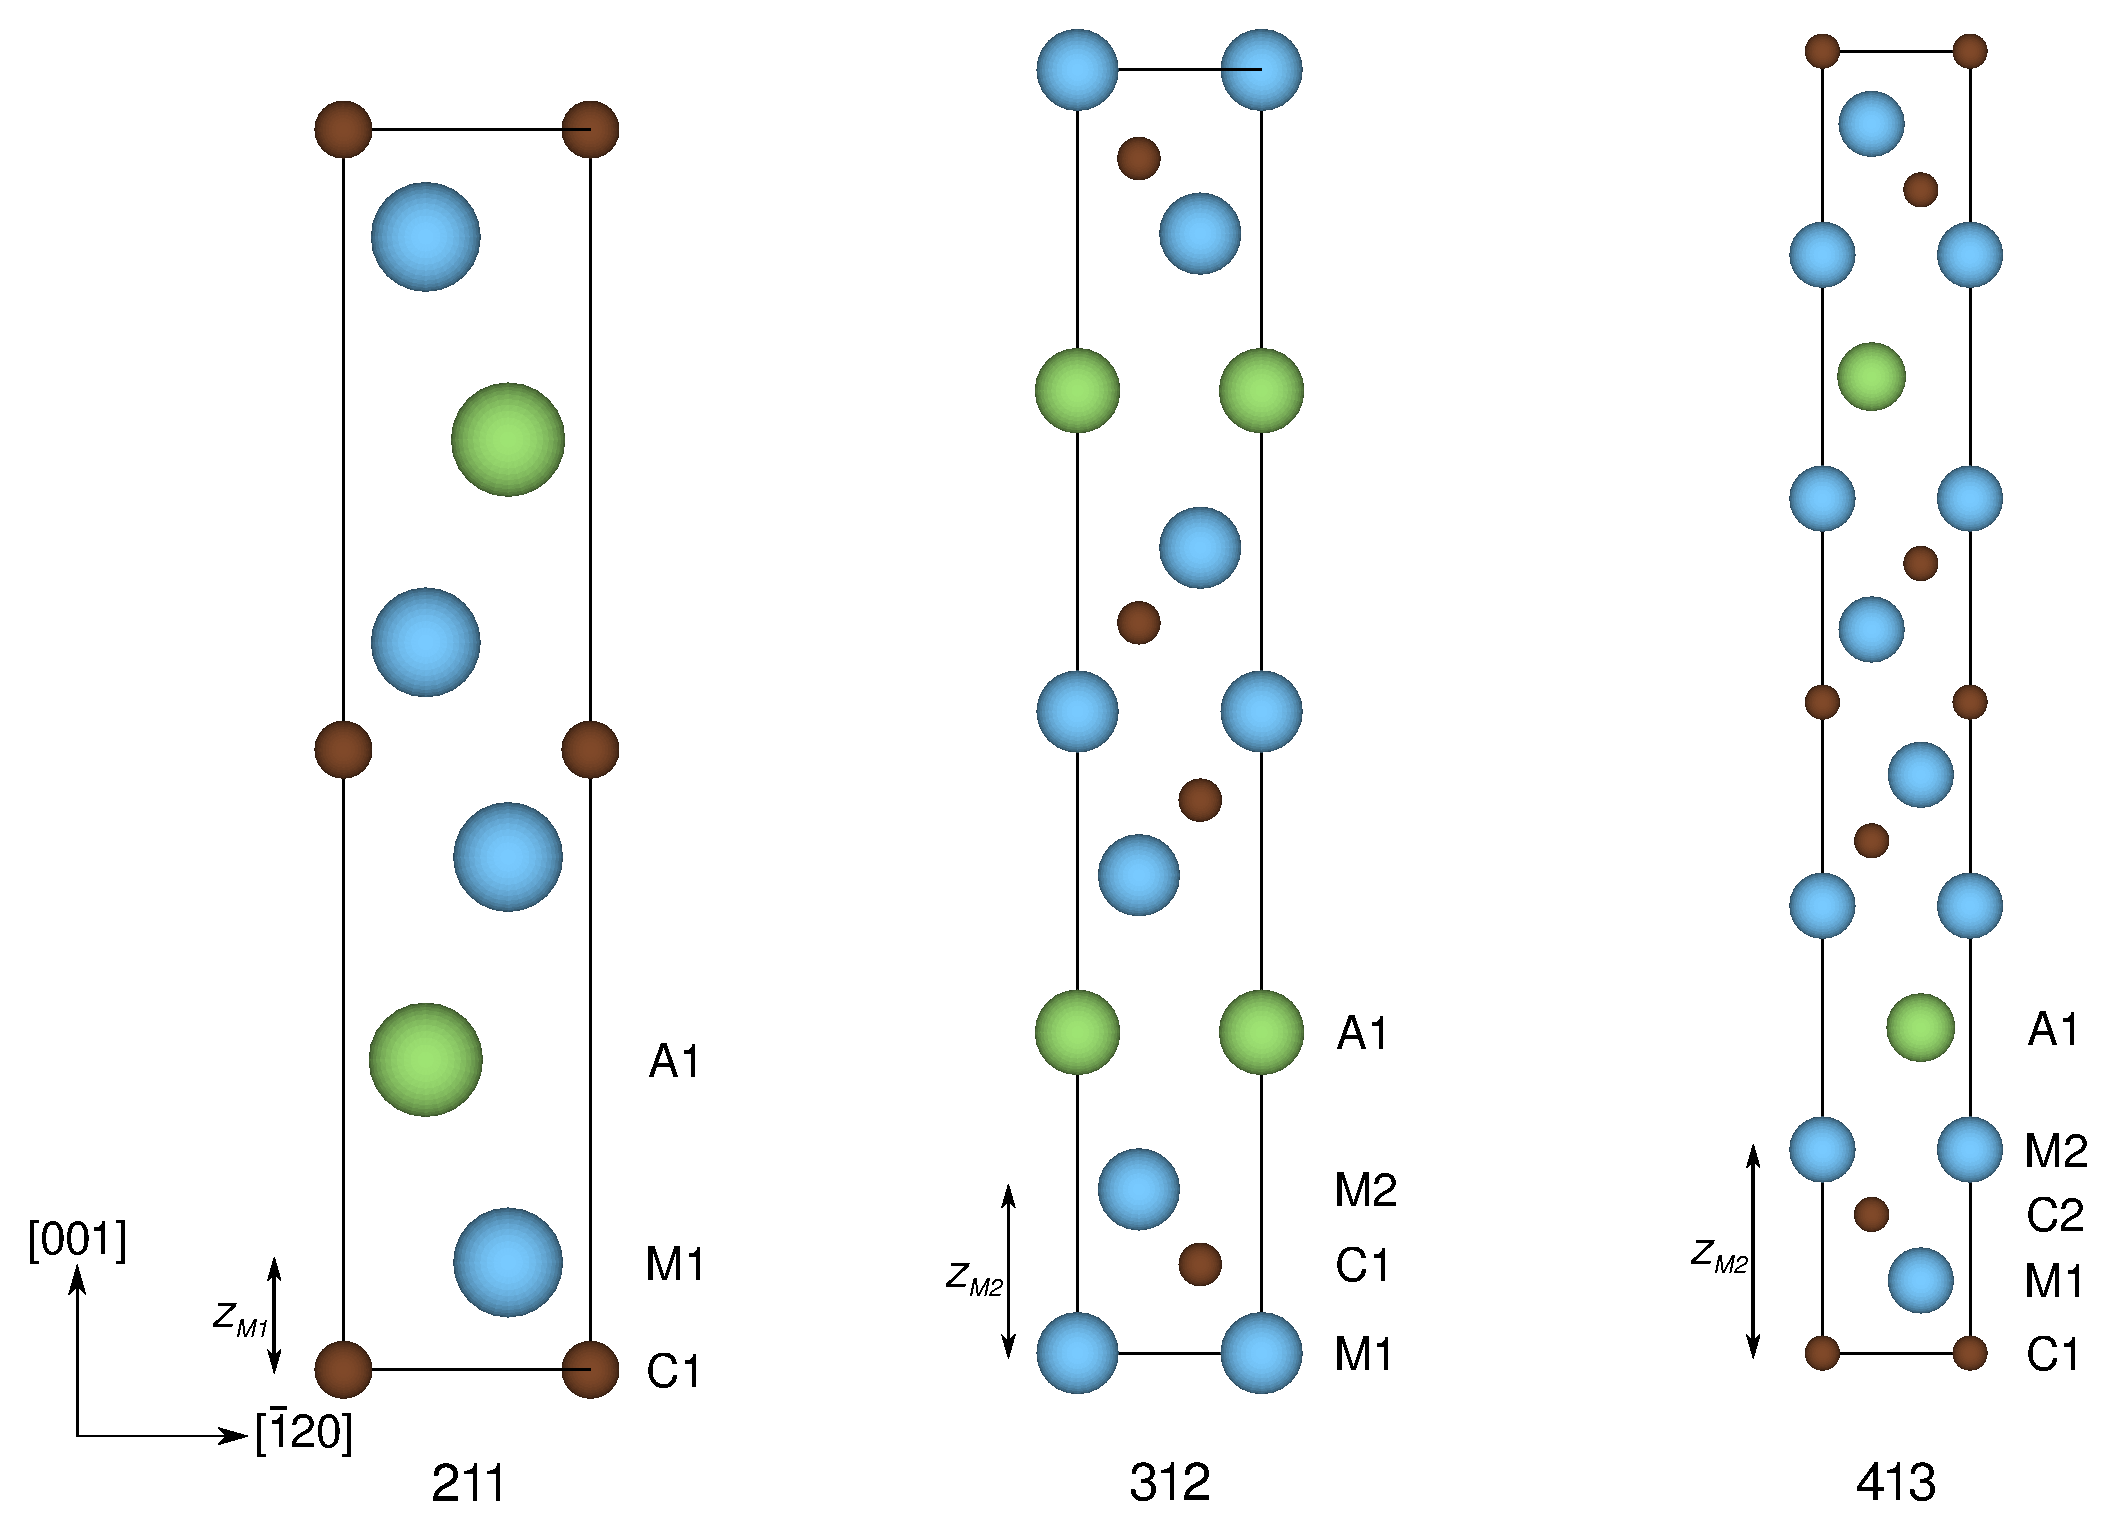
\includegraphics[width=\textwidth]{MAX_unit_cells}
\caption[The MAX phase unit cells.]{The unit cells of the first three possible MAX phases. Graphics prepared with VESTA \cite{Momma2011}.\label{fig:MAX_unit_cells}}
\end{figure}




\begin{figure}
\centering
\captionsetup{width=0.6\textwidth,font={sf,scriptsize},labelfont=bf}
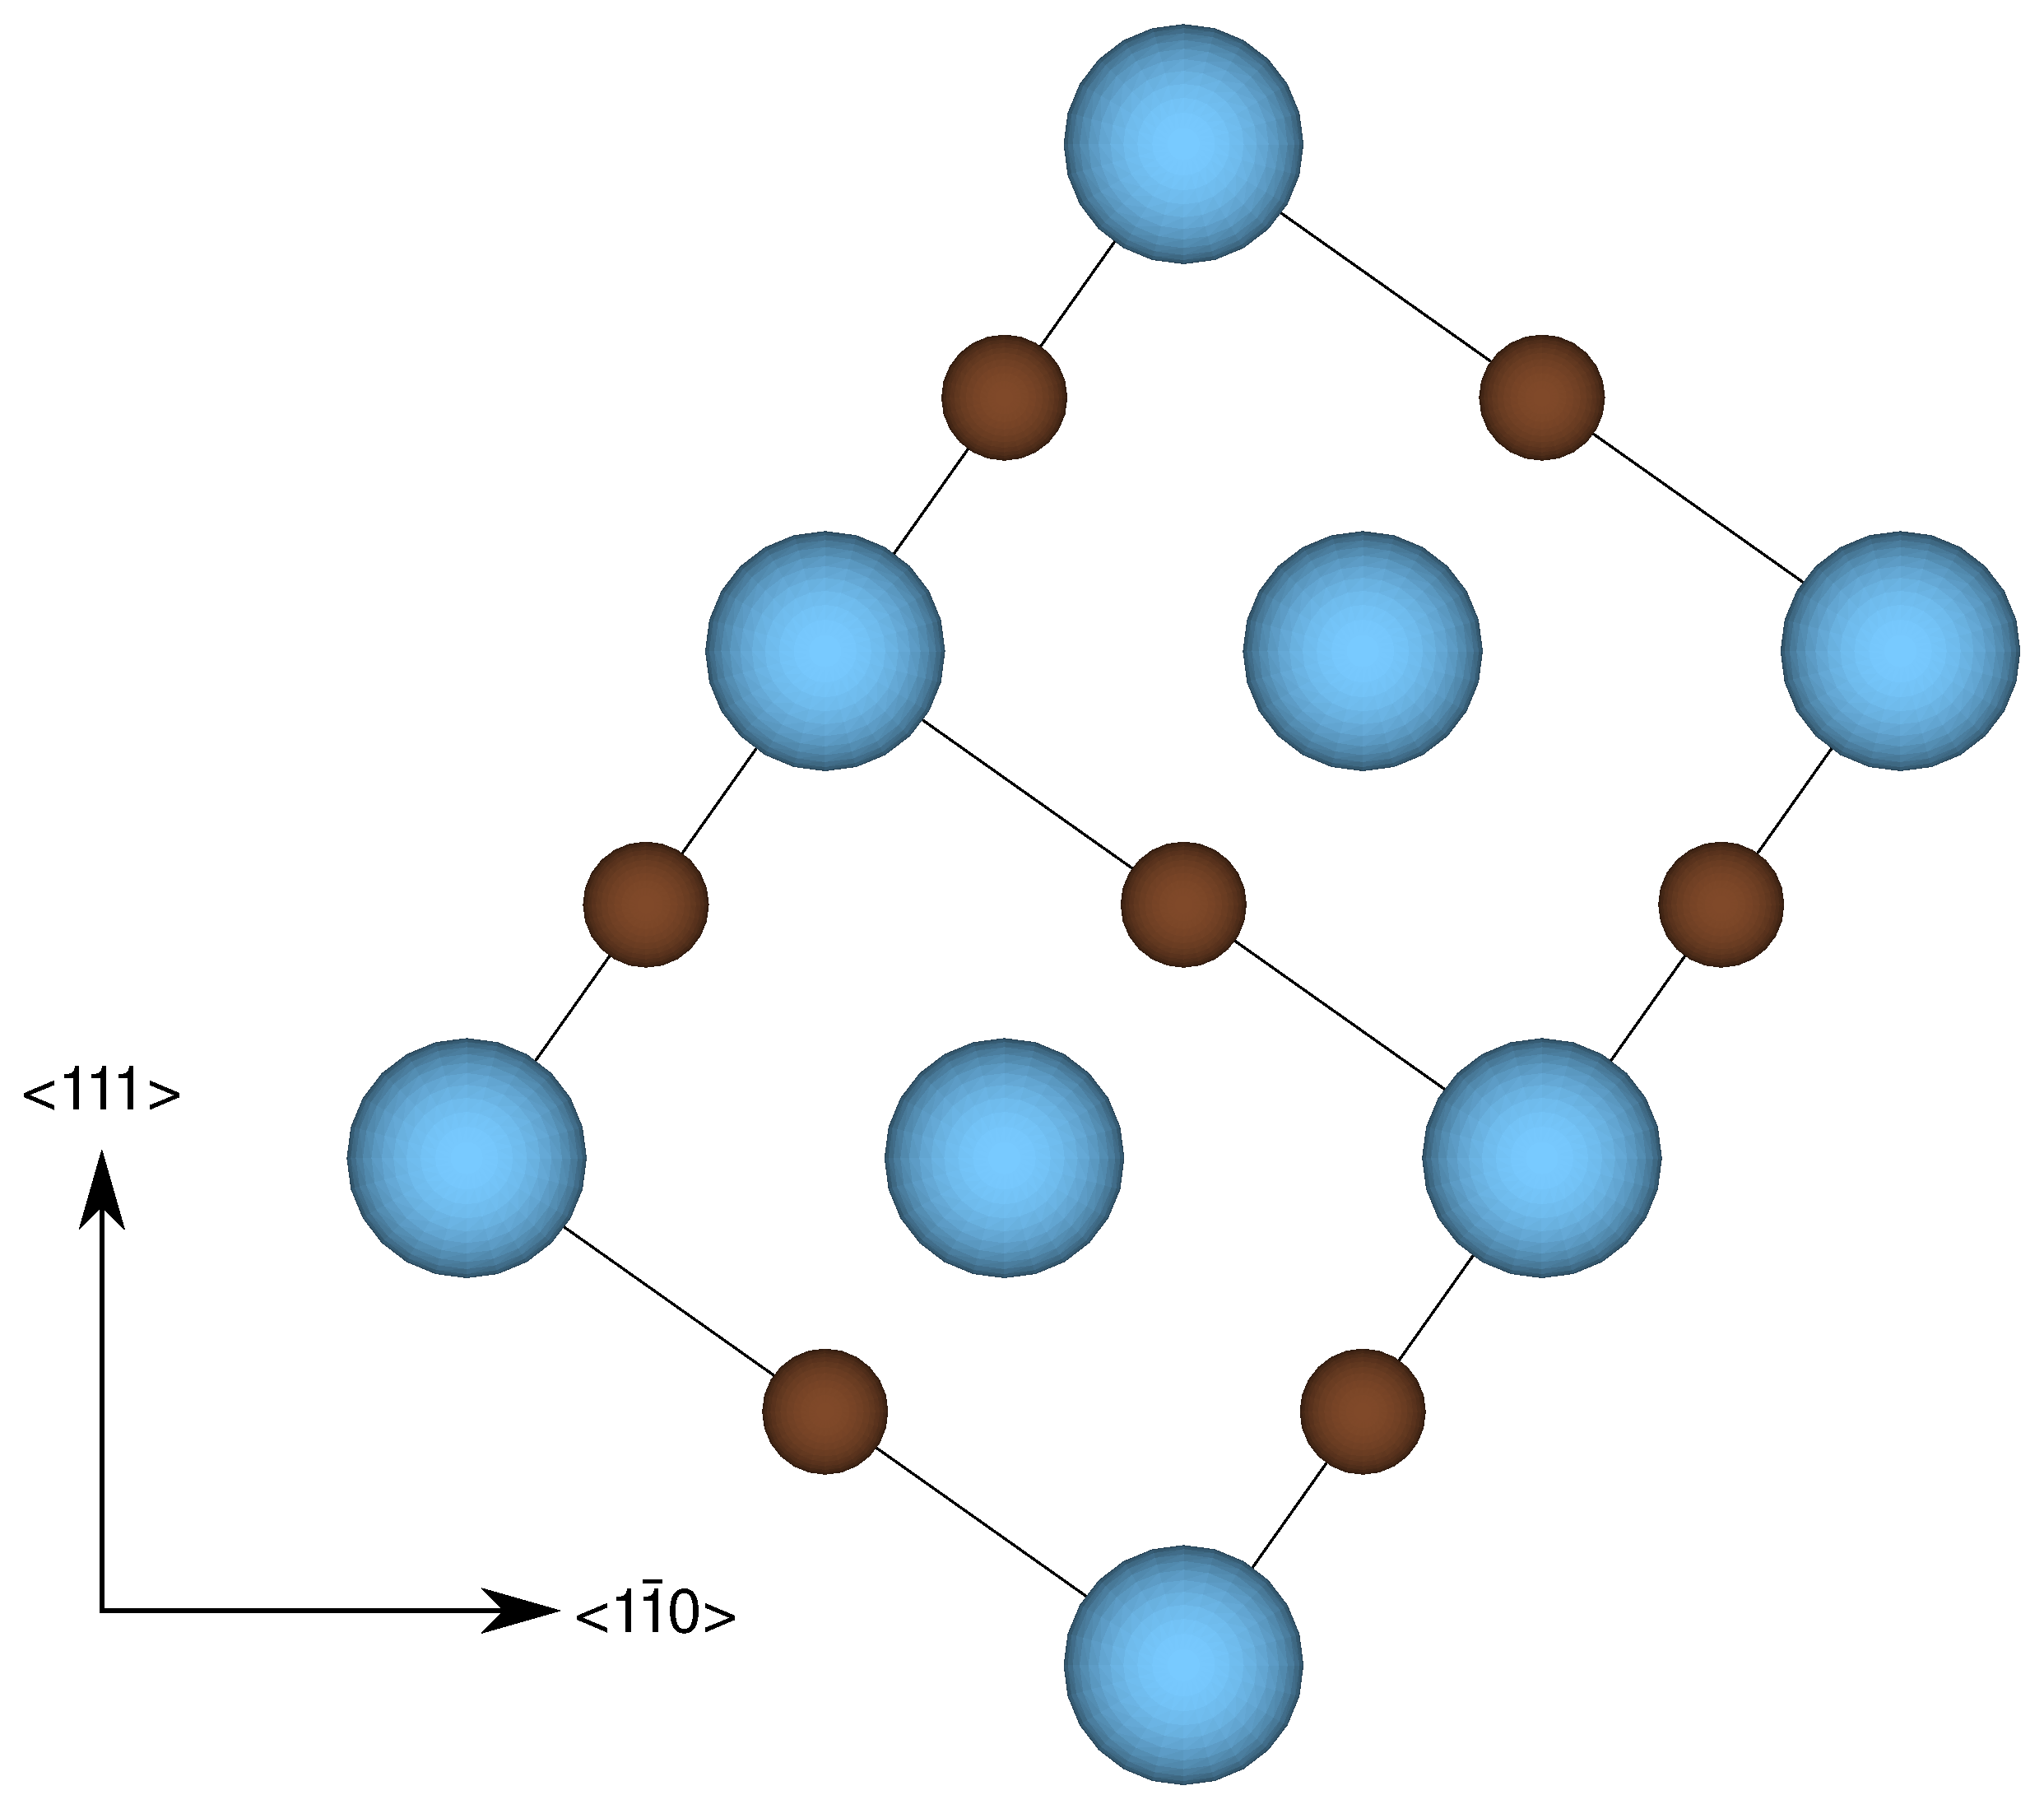
\includegraphics[width=0.5\textwidth]{TiC_111}
\caption[The unit cell of \ce{TiC}.]{The unit cell of \ce{TiC}, which has the rock salt structure, oriented to show the \{1\,1\,1\} planes which are equivalent to the MX layers of the MAX structure shown in \autoref{fig:MAX_unit_cells}. Graphic prepared with VESTA \cite{Momma2011}.\label{fig:TiC_111}}
\end{figure}


The description of complex crystals is often in terms of clusters of atoms that appear to pack together and fill space. The clusters may or may not have physical significance: for example clusters of up to 55 atoms of \ce{Ni}-\ce{Al} are stable on surfaces and so are clearly physically significant, but geometric descriptions of clusters can be made of simple materials like FCC aluminium \cite{Steurer2006}. Care must be taken therefore not to ascribe undue significance to purely geometric features, but the description of the MAX crystal structure as layers is not simply geometric but can be justified on the basis of heterogeneity in the chemical environments, i.e. the layers are meaningful.

The bonding in MAX phases has been shown, by density functional theory (DFT) calculations, to be a combination of metallic, covalent and ionic bonding but with covalent bonding predominant in the MX layer and metallic bonding in MA layers. Large variations in structural and mechanical properties are observed to depend on changes in the nature of this heterogeneous bonding character \cite{Radovic2013,Sun2011}. Notably the extreme (among MAX phases) properties of \ce{Ti2SC} are ascribed to the unusual strong bonding between \ce{Ti} and \ce{S} in addition to the strong bonding between \ce{Ti} and \ce{C} in contrast with most other MAX phases. This unusual bonding is taken to underlie the high elastic constants, $E =$~\SI{316}{\giga\pascal} the highest of any 211 MAX phase, and hardness of \SI{8}{\giga\pascal}, very nearly the highest of any bulk MAX phase \cite{Feng2010,Sun2011}.

\subsection{Deformation in MAX phases}

Deformation in \ce{Ti3SiC2} has been widely studied, particularly by Barsoum \cite{Farber1998,Barsoum1999,Farber1999,Barsoum1999dislocs_kinkbands,Barsoum2001}, and was found to readily occur by the glide of dislocations. Room temperature deformation was shown to increase the density of perfect basal dislocations with a Burgers vector equal to the lattice parameter $a$, so $b =$~<1\,1\,\={2}\,0>. 

Using heavily textured bulk samples of \ce{Ti3SiC2} the critical resolved shear stress of \ce{Ti3SiC2} was estimated by compression test. A sample with the basal planes of the sample oriented at approximately \SI{65}{\degree} to the compression axis and a yield stress of \SI{200}{\mega\pascal} was measured. Schmid's law is 

\begin{equation}
\tau_y = \sigma_y \cos{\phi} \cos{\lambda}
\end{equation}

where $\tau_y$ is the shear yield stress on the slip plane in question, $\sigma_y$ is the uniaxial yield stress\ $\phi$ is the angle between the slip plane normal and the loading axis, and $\lambda$ is the angle between the slip direction and the loading axis. The $\phi$ must be \SI{25}{\degree} ($=\SI{90}{\degree} - \SI{65}{\degree}$) but $\lambda$ is not known but if taken to be the maximum possible value, given $\phi=\SI{25}{\degree}$, of \SI{115}{\degree} then $\tau_y = \SI{77}{\mega\pascal}$, providing an upper bound \cite{Humphrey2012}. While this is higher than the estimate made by the original authors \cite{Barsoum1999}, \citet{Humphrey2012} points out that this is likely an overestimate due to the variation in Schmid factor across the sample and load redistribution between soft and hard grains but in any case is very low for a ceramic and approaches the flow stresses of pure cubic close-packed metals.


%%%%%%%%%%%%%%%%%%%%%%%%%%%%%%%%%%%%%%%%%%%%%%%%%%%%%%%%%%%%%%%%%%
%
%
%
%
%
%
% Figure about compression test here?
%
%
%
%
%
%
%%%%%%%%%%%%%%%%%%%%%%%%%%%%%%%%%%%%%%%%%%%%%%%%%%%%%%%%%%%%%%%


As discussed in \autoref{sec:tailor_peierls}, attempts have been made to explain and hence control the lattice resistance of materials, and this has been done for the MAX phases too. One study on MAX phases \cite{Music2007ductility} with the chemistry \ce{M2AlC} (M = Ti, V, Cr) used the more recent ductility criteria, namely Zhou-Carlsson-Thomson \cite{Zhou1994} and Rice \cite{Rice1992} which are discussed in detail in \autoref{sec:ductility_criteria}. There is recognition that the lattice resistance of a single dislocation, which is the limiting factor on ductility in most ceramics, is not simply dependent on bulk elastic constants. The authors therefore calculate ductility criteria based on stacking fault energies and surface energies, which necessitates choosing which plane to fault or cleave. In the MAX phases there are two natural choices: between the M atom and the A atom or between the M atom and the X atom. However there is no direct link, in these studies, between these properties and dislocation behaviour, and hence no direct link to the ductility. 

Some studies have considered the Peierls stress in complex crystals with layered structures \cite{Music2008,Emmerlich2009,Gouriet2015} but usually these have simply applied the result for an isotropic elastic material:
\begin{equation}
\tau_p = \frac{2G}{1-\nu} \exp \left( - \frac{2 \pi d}{b(1-\nu)} \right)
\end{equation}
where $G$ is the shear modulus, $\nu$ is the Poisson ratio, $d$ is the slip plane spacing and $b$ is the Burgers vector.


The result is therefore based on polycrystalline bulk elastic properties and the specifics of the MAX crystal structure are disregarded save the values of $d$ and $b$ chosen. These have tended to give high values of the Peierls stress, e.g. \SI{980}{\mega\pascal} for \ce{Ti2AlC} \cite{Music2008} which we can compare with \SI{700}{\mega\pascal} for \ce{TiC} \cite{Clegg2006}. The strength of \ce{TiC} should be an upper bound on the flow stress in the MAX phase, since the MAX phases contain planes of \ce{TiC}. Furthermore these planes of TiC in the MAX phases are equivalent to the slip planes in \ce{TiC} \cite{Hollox1966}. 

The GSF calculated by DFT has been used in at least one study \cite{Gouriet2015} but assumed that no change in confining elastic field occurred during dislocation motion, which has been shown to be significant \cite{Lubarda2007,Clegg2006}. \citet{Gouriet2015} also found Peierls stresses that are more similar to \ce{TiC}, of between \SI{611}{\mega\pascal} and \SI{957}{\mega\pascal}.

There is clearly a large effect of the crystal chemistry on the lattice resistance of the MAX phases which has not been adequately explained. If the effect can be understood it may allow a general route to tailoring the Peierls stress of a material and the introduction of a degree of ductility and toughness to otherwise brittle materials.
























































